% !TEX root = ../deviant.tex

\newcommand{\todofc}[1]{\todo[backgroundcolor=yellow,size=\tiny]{FC: #1}}
\newcommand{\todoinfc}[1]{\todo[inline,backgroundcolor=yellow]{FC: #1}}



\section{Experimental evaluation}
\label{sec:eval}

% Usually, an experimental evaluation of a process discovery algorithm would require to apply the proposed approach on one (or more) dataset, and to confront the learned model with those ones mined by other available approaches. However, our approach makes explicit use of information from traces labeled as ``negative'', while the totality of the approaches we could access have been designed to use positive traces only. Hence, confronting different approaches on different input data would not be fair.
% NO, questa motivazine non va bene...

One of the difficulties of evaluating process mining algorithms is that given a log, the underlying model might not be known before. As a consequence, it might be difficult to establish an \emph{ideal model} to refer and confront with. In this regard, a number of metrics and evaluation indexes have been proposed in the past to evaluate how a discovered model fits a given log \todofc{Citiamo qualche metrica? O forse basta citare un paper?}. However, those metrics provide only a partial answer to the question of ``how good'' is the discovered model.\todofc{Frase molto forte, la vogliamo lasciare? Forse dovremmo almeno citare un paper che dica qualcosa di simile\ldots Notate che siccome andiamo a fare coverage del 100\%, alcune metriche ci potrebbero premiare col massimo\ldots}

In the case of our approach, a further issue influences the evaluation process: the difficulty of performing a ``fair'' comparison with existing techniques, especially if we consider that our approach exploits information from traces labeled as ``negative'', while the majority of the methods we could access have been designed to use positive traces only.


%A second issue is about the difficulty of confronting our approach with existing ones, especially if we consider that \todofc{Non so se questa cosa la voglio scrivere qui\ldots} our approach exploits information from traces labeled as ``negative'', while the majority of the approaches we could access have been designed to use positive traces only.

We pursued two different evaluation strategies. On one side, we defined a model, and from that model we generated a synthetic, artificial log, having care that it exhibits a number of desired properties: in a sense, this part of the evaluation can be referred as being about a ``controlled setting''. A first aim is to understand if our approach succeeds to discover a \emph{minimum} set of constraints for distinguishing positive from negative traces; a second aim is to qualitatively evaluate the discovered model, having the possibility to confront it with the original one. Experiments conducted on that synthetic log are reported and discussed in Section \ref{sec:syntheticlog}.

On the other side, we applied our discovery technique to some existing logs, thus evaluating it on some real data set. Again, this experiment has two aims: to understand weakness and strengths of our proposal w.r.t. to some relevant literature; and to confront the proposed approach with real-world data---and difficulties that real-world data bring along. Section \ref{sec:realdata} is devoted to present the selected logs and discuss the obtained results.

% Such aspect is further exacerbated by the fact that our approach exploits information from traces labeled as ``negative'', while the totality of the approaches we could access have been designed to use positive traces only.



\subsection{Experiments on a synthetic dataset}
\label{sec:syntheticlog}

% PER REFERENCE INTERBA NOSTRA:
%
% init(receive_loan_application)
% existence(assess_eligibility)
% precedence(assess_loan_risk, assess_eligibility)
% precedence(appraise_property, assess_eligibility)
% exclusive_choice(reject_application, send_acceptance_pack)
% precedence(assess_eligibility, reject_application)
% precedence(assess_eligibility, send_acceptance_pack)
% not_coexistence(reject_application, notify_approval)
% not_coexistence(receive_positive_feedback, receive_negative_feedback)
% exclusive_choice(send_acceptance_pack, receive_negative_feedback)
% precedence(appraise_property, assess_loan_risk)

% existence(0, 1, appraise_property)
% existence(0, 1, check_credit_history)
% existence(0, 1, check_income_sources)
% existence(0, 1, assess_loan_risk)
% , assess_eligibility % rimosso perché è già oggetto di un vincolo existence...
% existence(0, 1, reject_application)
% existence(0, 1, send_acceptance_pack)
% existence(0, 1, verify_receipt)
% existence(0, 1, cancel_application)
% existence(0, 1, notify_cancellation)
% existence(0, 1, approve_application)
% existence(0, 1, notify_approval)
% existence(0, 1, ask_for_customer_feedback)
% existence(0, 1, receive_positive_feedback)
% existence(0, 1, receive_negative_feedback)

The synthetic log has been generated starting from a Declare model, using the tool \cite{2020-Loreti}. The model has been inspired by the Loan Application process reported in \textcolor{red}{(2018, Dumas)}. \todofc{Se abbiamo bisogno di spazio, la descrizione in NL del processo può essere saltata, e rimandiamo il lettore direttamente al disegno.} In our model, the process starts when the \emph{loan application} is received. Before \emph{assessing the eligibility}, the bank proceeds to \emph{appraise the property} of the customer, and to \emph{assess the loan risk}. Then, the bank can either \emph{reject the application} or \emph{send the acceptance pack} and, optionally, \emph{notify the approval} (if not rejected). During the process execution the bank can also \emph{receive positive} or \emph{negative feedback} (but not both), according to the experience of the loan requester. It is not expected, however, that the bank receives a \emph{negative feedback} if the \emph{acceptance pack} has been sent. Moreover, due to temporal optimization, the bank requires that the \emph{appraise of the property} is done before \emph{assessing the loan risk}.
To ease the understanding of the loan application process, a Declare model of the process is reported in Fig. \ref{fig:ex}. Moreover, all the activities have been constrained to either not be executed at all, or to be executed at most once: in Declare terminology, all the activities have been constrained to \emph{absence2}.

\begin{figure}[t]
\centering
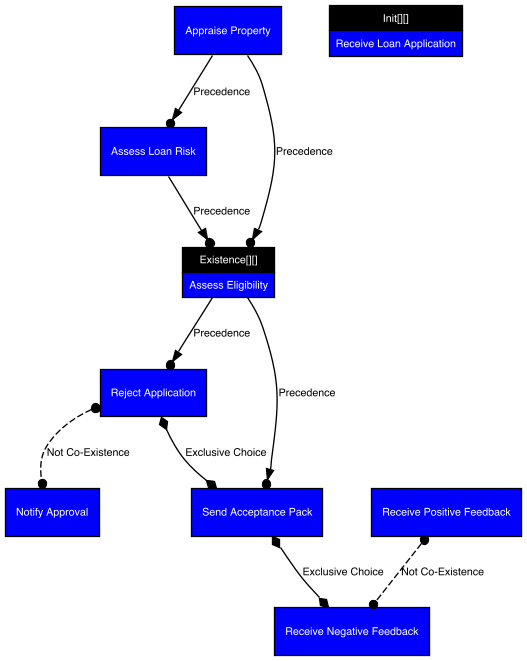
\includegraphics[width=0.6\columnwidth]{example1}
\caption{Loan approval declare process model }
\label{fig:ex}
\end{figure}

To test our approach, besides positive traces, we generated also negative traces. In particular, we generated traces that violate two different constraints:
\todofc{Non ho messo il terzo test di violazione, perch\`e riguardava ancora una \emph{precedence}\ldots pensiamo se vogliamo aggiungerlo.}
\begin{enumerate}[label=(\alph*)]
\item the \emph{precedence(assess\_loan\_risk, assess\_eligibility)}, that is violated when either the latter activity is executed and the former is absent, or if both the activities appear in the log, but in the wrong temporal order;
%
\item the \emph{exclusive\_choice(send\_acceptance\_pack, receive\_negative\_feedback)}, that is violated when a trace either contains both the activities, or does not contain any of them.
\end{enumerate}
%
The resulting log consists of 64,000 positives traces, 25,600 traces that violates the constraint as in $(a)$, and 10,240 traces that violates the constraint as specified in $(b)$.
%
When fed with the positives traces and traces violating the constraint in $(a)$, our approach successfully manages to identify constraints that allow to clearly distinguish positives from negatives traces. Moreover, the discovered constraint coincides with the one we originally decided to violate during the generation phase. When confronted with the $(b)$ scenario, our approach again successfully managed to identify a minimum model able to discriminate between positive and negative traces, and the identified constraint is indeed logically consistent with the constraint originally selected for the violation.
% In particular, it is worthy to notice that our approach derived 
Table \ref{tab:syntResults} summarize the obtained results and reports the first selected model for each scenario.

% source of this data:
% file:///Users/federico/Google%20Drive/on-negative-traces/experiments/2020-07-14%20Federico/run_experiments_2020-07-30_130357_CEST.html
\begin{table}
\tiny
\begin{tabular}{c c c c p{3cm} | p{3cm}}
\hline
Scenario & \#pos & \#neg & time & Originally violated constraint & Discovered model \\
\hline\hline
$(a)$ & 64,000 & 25,600 & \bf{Total: \fpeval{81.78 + 1.94 + 109.74 + 3.32 + 15.165}s} & \emph{precedence(assess\_loan\_ risk, assess\_eligibility)} & \emph{precedence( assess\_loan\_risk, assess\_eligibility)}\\
& & & Compatibles:  \fpeval{81.78 + 1.94}s  & & \\
& & & Choices:  \fpeval{109.74 + 3.32}s  & & \\
& & & Optimisation: 15.165s & & \\
%
\hline
%
$(b)$ & 64,000 & 10,240 & \bf{Total: \fpeval{81.78 + 1.94 + 94.51 + 2.96 + 1.379}s} & \emph{exclusive\_choice( send\_acceptance\_pack, receive\_negative\_ feedback)} & \emph{coExistence(reject\_application, receive\_negative\_feedback)}\\
& & & Compatibles:  \fpeval{81.78 + 1.94}s  & & \\
& & & Choices:  \fpeval{94.51 + 2.96}s  & & \\
& & & Optimisation: 1.379s & & \\
\hline
\end{tabular}
\caption{Models discovered when dealing with the synthetic data set.}
\label{tab:syntResults}
\end{table}


% PARAMETRI RuM usati:
% Templates: devi selezionarli tutti eccetto:
%  - not precedence
%  - not chain precedence
%  - not response
%  - not chain response
%  - not responded existence
% Constraint support: io ho provato 80,90 e 100 - qui penso che puoi vedere un po' in base ai risultati che ti escono
% Pruning types: come dicevo oggi li ho provati tutti e 4 ma secondo me e` sufficiente None.
% Vacuity detection: deve essere OFF
% Activity support filter: deve essere a 0%



\todoinfc{ChiaraDFM, qui ci starebbe bene un paragrafetto in cui riportiamo i risultati ottenuti usando RuM. Il commento che potremmo scrivere e' che RuM trova un modello intero per coprire le positive, e riesce a distingure benissimo anche le negative: il risultato e' atteso, dato l'elevato numero di tracce che rende il synthetic data set molto informativo.}
% Beside positive trace, we also generated negative traces in a controlled way, i.e. taking care that those traces violate only a small, specific and known piece of the model.

% \todoinfc{x Fede, Chiara DFM, Sergio: qui bisognerebbe introdurre la metodologia per provare la validit\`a del nostro approccio, cio\`e abbiamo preso questo esempio, abbiamo generato delle tracce (cit \cite{2020-Loreti}), alcune positive, altre negative che per\`o violano dei vincoli che in questo modello non sono presenti e poi abbiamo visto se riusciamo a re-impararli. Perch\`e proprio questi vincoli e non altri?}

% A bank carries out the following \emph{loan application} process\footnote{The process is inspired by the Loan Application process reported in (2018, Dumas).} in order to grant loans. The process starts when the \emph{loan application} is received. In order to decide whether to \emph{reject the application} or to \emph{send the acceptance pack} to the customer for receiving the customer's official acceptance, the bank has to \emph{assess} the \emph{eligibility} of the loan. To this aim, the customer's \emph{property} has to be \emph{appraised} and the \emph{loan risk assessed} by the bank. The bank can optionally \emph{notify} the customer about the loan \emph{approval}, of course in case the loan is not rejected. During the process the bank can also \emph{receive positive} or \emph{negative feedback} according to the experience of the loan requester. To ease the understanding of the loan application process, a Declare model of the process is reported in Fig. \ref{fig:ex}.


% Among the processed loan application requests, some are considered as negative by the bank, while others as positive. In detail, the negative cases are the ones in which:
% \begin{itemize}
% \item the bank receives a negative feedback, although the acceptance pack is sent to the customer;
% \item the time required for carrying out the whole procedure is huge (this happens when the property appraisal is performed after the loan risk assessment).
% \end{itemize}

% Being aware of the process executions that deviate from its expectations (the negative cases), the bank would like to discover a process model of the loan application procedure in which only the positive cases are included, while the deviant ones are excluded.

\subsection{Evaluation on case studies from real data}
\label{sec:realdata}

\todoindl{Chiara DFM\&Sergio\&Fabrizio: descrizione dataset e risultati di esperimenti coi dati veri}

For the experimentation with real datasets, we used three real-life event logs: \textsc{cerv}, \textsc{sepsis} and \textsc{bpic12}. Starting from these event logs we generated 5 different datasets, each composed of a set of positive and a set of negative traces, by applying different criteria to distinguish between positive and negative traces, i.e., by labeling the event log with different labeling functions. 

\textsc{cerv} is an event log related to the process of cervical cancer screening carried out in an Italian cervical cancer screening center~\cite{2007b-Lamma}. Cervical cancer is a disease in which malignant (cancer) cells form in the tissues of the cervix of the uterus. The screening program proposes several tests in order to early detect and treat cervical cancer. It is usually composed by five phases: Screening planning; Invitation management; First level test with pap-test; Second level test with colposcopy, and eventually biopsy. The traces contained in the event log have been analyzed by a domain expert and labeled as compliant (positive traces) or non-compliant (negative traces) with respect to the cervical cancer screening protocol adopted by the screening center.

\textsc{sepsis}~\cite{Sepsis} is an event log that records trajectories of patients with symptoms of the life-threatening sepsis condition in a Dutch hospital.
%Œ\textsc{Sepsis} is an event log that records trajectories of patients with symptoms of the life-threatening sepsis condition in a Dutch hospital. 
Each case logs events since the patient’s registration in the emergency room until her discharge from the hospital. Among others, laboratory tests together with their results are recorded as events. The traces contained in the event log have been labelled based on their cycle execution time. In the \textsc{sepsis$_{mean}$} dataset, traces with a cycle time lower than the mean duration of the traces in the event log ($\sim$ 28 days) have been labelled as positive, as negative otherwise. Similarly, in the \textsc{sepsis$_{median}$}, traces with a cycle time lower than the median duration of the traces in the event log ($\sim$ 5 days)  have been labeled as positive, as negative otherwise.  

\textsc{bpic12}~\cite{BPIC2012} is a real-life event log pertaining to the application process for personal loans or overdrafts in a Dutch financial institute. It merges three intertwined sub-processes. Also in this case, the traces have been labelled based on their cycle execution time. In the \textsc{bpic12$_{mean}$} dataset (resp. \textsc{bpic12$_{mean}$}), traces with a cycle time lower than the mean (resp. median) duration of the traces in the event log ($\sim$ 8 days, resp. $\sim$ 19 hours) have been labelled as positive, as negative otherwise. 

%The \textsc{cerv} event log has been labeled based on the compliance of th


Table~\ref{tab:rl_datasets} summarizes the data related to the five resulting datasets.

\begin{table} [h]
	\centering
	\scalebox{0.8}{
		\begin{tabular} {l l c c c c c}
		\toprule
			\multirow{2}{*}{\textbf{Dataset}} & \multirow{2}{*}{\textbf{Log}} & \multirow{2}{*}{\textbf{Trace \#}} & \multirow{2}{*}{\textbf{Activity \#}} & \multirow{2}{*}{\textbf{Label}} & \textbf{Positive} & \textbf{Negative}  \\ 
			& & & & & \textbf{Trace \#} & \textbf{Trace \#} \\ \midrule
			\textsc{cerv$_{compl}$} & \textsc{cerv} & 157 & 16 & compliant & 55 & 102 \\ \midrule
			\textsc{sepsis$_{mean}$} & \multirow{2}{*}{\textsc{sepsis}} & \multirow{2}{*}{1000} & \multirow{2}{*}{16} & mean duration & 838 & 212 \\
			\textsc{sepsis$_{median}$} &  &  &  & median duration & 525 & 525 \\ \midrule
			\textsc{bpic12$_{mean}$} & \multirow{2}{*}{\textsc{bpic12}} & \multirow{2}{*}{13087} & \multirow{2}{*}{36} & mean duration & 8160 & 4927  \\
			\textsc{bpic12$_{median}$} &  &  &  & median duration & 6544  & 6543 \\ 			
			\bottomrule
		\end{tabular}}
		\caption{Dataset description}
		\label{tab:rl_datasets}
\end{table}

Table~\ref{tab:rl_results} summarizes the results obtained by applying the \nd algorithm. In detail, the table reports for each dataset, (i) the results related to \minclos and \subsetclos - in terms of number of returned models\footnote{We stop generating models after $20$ models, i.e., \para{max} in Table~\ref{tab:rl_results} indicates that more than $20$ models have been returned.}, in terms of minimum size of returned models, as well as in terms of average percentage of negative traces excluded by the returned model. Moreover, the table reports the time required for computing the set of compatibles, the set of choices, as well as for \minclos and \subsetclos.

\begin{table} [h]
	\centering
	\scalebox{0.58}{
		\begin{tabular} {l | c c c | c c c | c c c c}
		\toprule
			\multirow{4}{*}{\textbf{Dataset}} & \multicolumn{3}{c|}{\textbf{\minclos}} & \multicolumn{3}{c|}{\textbf{\subsetclos}} & 	\multicolumn{4}{c}{\textbf{ Required Time (s)}} \\ \cmidrule{2-11}
			& \textbf{Number} & \textbf{Min} & \textbf{Avg.} & \textbf{Number} & \textbf{Min} & \textbf{Avg.} & \multirow{3}{*}{\textbf{Comp.}} & \multirow{3}{*}{\textbf{Choices}} & \multirow{3}{*}{\textbf{\minclos}} & \multirow{3}{*}{\textbf{\subsetclos}} \\			
			& \textbf{of} & \textbf{model} & \textbf{Violated} & \textbf{of} & \textbf{model} & \textbf{Violated} & & & & \\
			& \textbf{models} & \textbf{size} & \textbf{L$^{-}$ \%} & \textbf{models} & \textbf{size} & \textbf{L$^{-}$ \%} & & & & \\\midrule
			\textsc{cerv$_{compl}$} & \para{max} & 4 & 100\% & \para{max} & 4 & 100\% & 0.12 & 0.33 & 0.045 & 0.065 \\ \midrule
			\textsc{sepsis$_{mean}$} & 1 & 8 & 4.25\% & 1 & 8  & 4.25\% & 0.73 & 1.04 & 0.035 & 0.039 \\ 
			\textsc{sepsis$_{median}$} & 16 & 14 & 26.86\% & \para{max} & 14 & 26.86\% & 0.45 &	1.5 & 0.087 & 0.2 \\ \midrule
			\textsc{bpic12$_{mean}$} & \para{max} & 12 & 1.42\% & \para{max} & 12 & 1.42\% & 13.51 & 31 & 0.066 & 0.096  \\ 
			\textsc{bpic12$_{median}$} & \para{max} & 22 & 36.59\% & \para{max} & 23 & 36.59\% & 13.32 & 37.63 & 43.846 & 359.164 \\ 			
			\bottomrule
		\end{tabular}}
		\caption{Real Life log results}
		\label{tab:rl_results}
\end{table}

The table shows that for the \textsc{cerv$_{compl}$} dataset, \nd is able to return models that satisfy the whole set of positive traces and violate the whole set of negative traces (the percentage of violated traces in $L^-$ is equal to 100\%) with a very low number of constraints (4). For the other datasets, the returned models are always able to satisfy all the traces in $L^+$, however not all the negative traces are violated by the returned models. In case of the datasets built by using the mean of the trace cycle time, the percentage of violated traces is relatively small ($4.25\%$ for \textsc{sepsis$_{mean}$} and $1.24\%$ for \textsc{bpic12$_{mean}$}), as the number of constraints of the returned models ($8$ for \textsc{sepsis$_{mean}$} and $12$ for \textsc{bpic12$_{mean}$}). Nevertheless, \nd is able to obtain reasonable results with the real life datasets built with the median of the trace cycle time. Indeed, it is able to return models able to accept all the traces in $L^+$ and to cover about $27\%$ (resp. $37\%$) of the traces in $L^-$ for \textsc{sepsis$_{median}$} (resp. \textsc{bpic12$_{median}$}). The difference in terms of results between the  \textsc{cerv$_{compl}$} and the other datasets is not surprising. Indeed, while what characterizes positive and negative traces in the \textsc{cerv$_{compl}$} dataset depend upon the control flow (i.e., it depends on whether each execution complies with the cervical cancer screening protocol adopted by the screening center), when mean and median cycle time are used, the difference between positive and negative traces could likely not exclusively depend on the control flow of the considered traces. \todocdf{I would add the language bias in the discussion.}
The table also shows that \nd is overall very fast for small datasets (e.g., less than one minute for \textsc{cerv$_{compl}$}), while it requires some more time for large ones (e.g., \textsc{bpic12$_{mean}$} and \textsc{bpic12$_{median}$}). While the time required for computing \textit{compatibles} and \textit{choices} seems to be related to the size of the dataset, the time required for computing the closures seems to depend also on other characteristics of the datasets). 

We compared the obtained results with the ones obtained with state-of-the-art techniques for the discovery of declarative models starting (i) from  only positive traces; and (ii) from both positive and negative traces. 

%For the former case, we used the state-of-the-art Declare miner algorithm~\cite{2018a-Maggi}  implemented in the RuM toolkit~\cite{2020-Alman}. For the latter we compared the results obtained with \nd with the ones of DecMiner, the approach based on Inductive Logic Programming proposed in~\cite{2007b-Lamma}.

Concerning the classical declarative discovery from only positive execution traces, we used the state-of-the-art \declare miner algorithm~\cite{2018a-Maggi} implemented in the \rum toolkit~\cite{2020-Alman}. We used the \declareminer algorithm\footnote{We run the \declareminer algorithm with vacuity detection disabled, \par{activity support filter} set to 0\%, using both transitive closure and hierarchy-based reduction of the discovered constraints, as well as with all the Declare templates, except for \dec{NotResponse}, \dec{NotPrecedence}, \dec{NotChainPrecedence}, \dec{NotChainResponse}, \dec{NotRespondedExistence}.} to discover the \declare model starting from the only positive traces with different values of the \para{support} parameter, which measures the percentage of (positive) traces satisfied by the \declare model.  \todocdf{Move this part when the results are presented for the synthetic data}

Table~\ref{tab:rl_declare_miner} summarizes the obtained results. In detail, the table reports for each dataset and \para{support}, i.e., percentage of positive traces satisfied by the model, the size of the model in terms of number of constraints, as well as the percentage of negative traces violated by the model.

\begin{table} [h]
	\centering
	\scalebox{0.8}{
		\begin{tabular} {l l c c}
		\toprule
			\textbf{Dataset} & \textbf{\para{support}} & \textbf{Model size} & \textbf{Avg. violated L$^{-}$ \%}  \\ \midrule
			\multirow{2}{*}{\textsc{cerv$_{compl}$}} & 100\% & 323 & 9.8\% \\ 
			& 90\% & 517 & 100\% \\ \midrule
			\multirow{3}{*}{\textsc{sepsis$_{mean}$}} & 100\% & 210 & 4.25\%\\
			& 95\% & 342 & 81.13\% \\
			& 90\% & 363 & 100\% \\ \midrule
			\multirow{3}{*}{\textsc{sepsis$_{median}$}} & 100\% & 202 & 22.29\% \\ 
			& 95\% & 211 & 88.19\% \\
			& 90\% & 322 & 100\% \\ \midrule
			\multirow{3}{*}{\textsc{bpic12$_{mean}$}} & 100\% & 514 & 0\% \\
			& 90\% & 637 & 83.52\%\\ 
			& 80\% & 650 & 100\%\\ \midrule
			\multirow{3}{*}{\textsc{bpic12$_{median}$}} & 100\% & 532 & 14.21\% \\ 
			& 80\% & 654 & 98.18\% \\			
			& 60\% & 654 & 98.18\% \\	
		\bottomrule
		\end{tabular}}
		\caption{\declareminer results}
		\label{tab:rl_declare_miner}
\end{table}

Finally, we compared the results obtained with \nd with the ones of \decminer, the state-of-the-art approach using both positive and negative execution traces based on Inductive Logic Programming proposed in~\cite{2007b-Lamma}. To this aim, we run the same procedure described in~\cite{2007b-Lamma} on the same dataset (the \textsc{cerv$_{compl}$} dataset) used in the same paper. Five fold-cross validation was used, i.e., the \textsc{cerv$_{compl}$} dataset was divided into 5 sets and in each experiment 4 were used for training and the remaining one for testing. The average accuracy of the five executions is collected, where the accuracy is defined as the sum of the number of compliant traces that are correctly classified as compliant by the learned model and the number of non-compliant traces that are correctly classified as non-compliant by the learned model divided by the total number of traces. Table~\ref{tab:acc_results} reports the obtained accuracy values for the \decminer, the \declareminer (with different values of the \para{support} parameter) and the \nd (both for the \minclos and \subsetclos closure) approach.

\begin{table} [h]
	\centering
	\scalebox{0.8}{
		\begin{tabular} {l c c}
			\toprule
			 \decminer &  & 97.44\%\\ \midrule
			\multirow{3}{*}{\declareminer} & \para{support}=100\% & 48.53\%\\
			& \para{support}=90\% & 95.5\% \\
			& \para{support}=80\% & 96.15\% \\ 
			& \para{support}=10\% & 81.94\% \\ \midrule
			 \multirow{2}{*}{\nd} & \minclos & 97.57\% \\ 
        & \subsetclos & 97.38\% \\ 			
			\bottomrule
		\end{tabular}}
		\caption{Accuracy results obtained with \declareminer, \decminer and \nd}
		\label{tab:acc_results}
\end{table}




